\documentclass[a4paper, 14pt]{article}
\usepackage{comment}

\usepackage{setspace}
\usepackage{indentfirst}
%% Language and font encodings
\usepackage{extsizes}
\usepackage[english, russian, ukrainian]{babel}
\usepackage[utf8x]{inputenc}
\usepackage[T1]{fontenc}
\linespread{1.6}
%% Sets page size and margins
\usepackage[a4paper,top=2cm,bottom=2cm,left=3cm,right=2cm,marginparwidth=1.75cm]{geometry}

%\usepackage{fontspec}

%% Useful packages
\usepackage{authblk}
\usepackage{amsmath}
\usepackage{graphicx}
\usepackage[colorinlistoftodos]{todonotes}
\usepackage[colorlinks=true, allcolors=black]{hyperref}
\usepackage{tikz}
%\usepackage{subfigure}
\usepackage[lofdepth,lotdepth]{subfig}
\usepackage{float}
\usepackage{multirow}
\usepackage{hhline}
\usepackage{lineno}

%\linenumbers
\renewcommand{\thefigure}{\thesection.\arabic{figure}}

\numberwithin{equation}{section}
\numberwithin{table}{section}

\title{}


\author[1]{V. Haponov}
\author[2]{R. Yermolenko}
\affil[1]{Taras Shevchenko National University of Kiev, Kiev, Ukraine}
\affil[2]{}

\setcounter{Maxaffil}{0}
\renewcommand\Affilfont{\itshape\normalsize}
\renewcommand{\arraystretch}{1.5} %% increase table row spacing
%\renewcommand{\tabcolsep}{1cm}

\date{}
\begin{document}
	
%title page
\begin{titlepage}
\renewcommand{\baselinestretch}{1.0}
\selectlanguage{ukrainian}
\begin{center}
	КИЇВСЬКИЙ НАЦІОНАЛЬНИЙ УНІВЕРСИТЕТ ІМЕНІ ТАРАСА ШЕВЧЕНКА\\Фізичний факультет\\Кафедра ядерної фізики
\end{center}
\vspace*{1.5cm}

\vspace*{3cm}
\begin{center} {\bf Використання сгорткових нейроних мереж для покращення точності аналізу результатів вихрострумового контролю}
\end{center}

\renewcommand{\baselinestretch}{1.5}
\vspace*{9cm}
{}\hfill\hspace{7.5cm}\parbox{9cm}{\textbf{Звіт з наукової практики}\\
	студента 1 курсу магістратури \\ Гапонова Валентина Вікторовича \\ \\ 
	\textbf{Науковий керівник} \\ канд. ф.-м. наук\\ Єрмоленко Руслан Вікторович}
\bigskip
\end{titlepage}
%end

%content
\selectlanguage{ukrainian}
\newpage
\tableofcontents
\newpage
\pagestyle{plain}
\setcounter{page}{2}
%end 

\section{Результати}

\subsection{Вихрострумовий контроль}
Було проведенно дослідження та аналіз використання вихроструммового контролю для неруйнівного аналізу, зокрема для нейруйнівного контролю титанових пластин, з використання глибоко навчання нейронних мереж. \\
Розрахунок середньої глибини проникання:
$$\delta = \frac{1}{\sqrt{\pi f \mu_0 \mu_r \sigma}}$$
Стандартна глибина проникання – відстань в провіднику на якій вихрові струми мають величину 36.8\% - їх величини на поверхні\\
Частота струму в генераторі обернено пропорційна глибині проникання \\
Глибині проникання обернено пропорційна  магнітній та електричній проникності середовища  
\subsection{Використання згорткових нейроних мереж}
За останні роки згорткові нейронні мережі гарно себе проявили для аналізу зоображенняб тому в подальшому буде розглянуто два випадки успішного застосування нейронних мереж для нейруйнівного контролю. 
В перешому з них результати вихростурмового контрою конвертувалися в зоображення, та запускалась нейронна мережа на основі тензорфлоу для визначення характеру та розмірів дефекту титаної пластини.
Результати порівняльної характеристики для різних нейронних мереж надані на Рис \ref{fig1}
\begin{figure}[htbp]
	\centerline{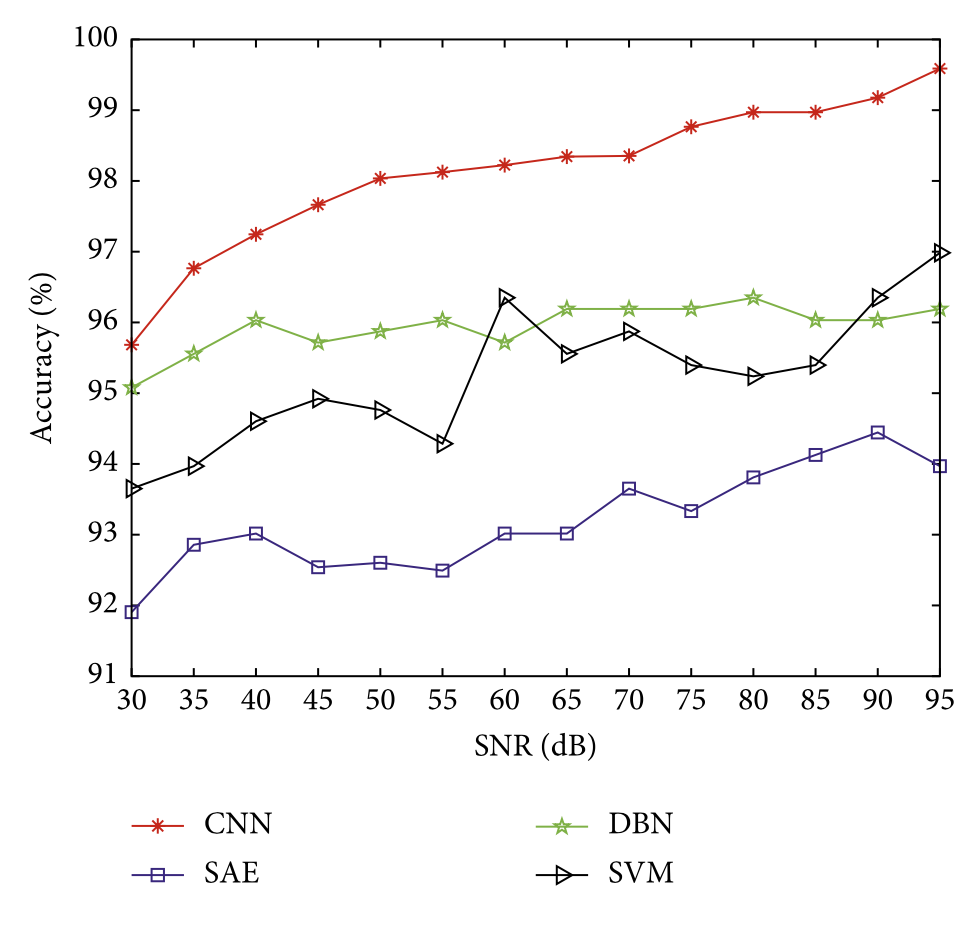
\includegraphics[scale=1]{res/image1.png}}
	\caption{Порівняльна характеристика точності нейронних мереж при різних ріівнях шуміві}
	\label{fig1}
\end{figure}
%
\newpage

\subsection{Сгорткові мережі для візуального пошуку дефектів}
\begin{figure}[htbp]
	\centerline{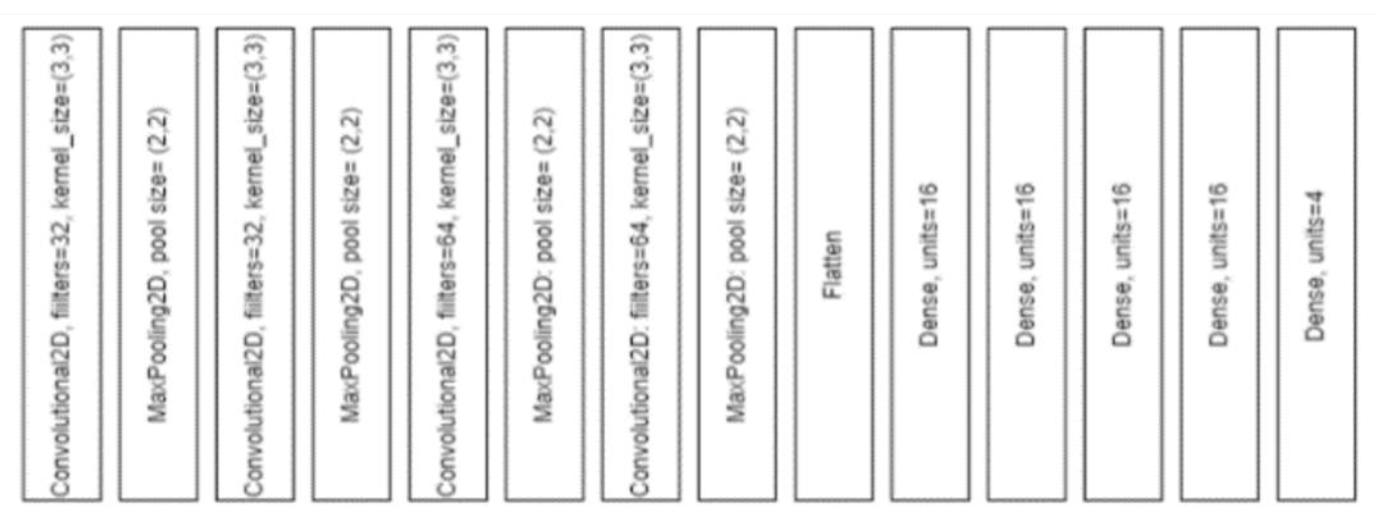
\includegraphics[scale=.7]{res/image4.png}}
	\caption{Архітектура нейроної мережі для візуального пошуку дефектів}
	\label{fig4}
\end{figure}

Мережа представлена на Рис \ref{fig4}, була створена за допомогою бібліотеки \"TensorFlow\". 
Данна мережа дозволила визначати наявність та загальний характер дефекту з точністб до 97.55\%, враховуючи, що вимірювальна здатність починаєтся з 16мм в довжину - для потреб ядерної фізики подібний дефект, являєтся значним. Тому використання нейронних мереж для візуального аналізу є не можливим\\
Не зважаючи на це враховуючи що в експеременті покладався рівень яскравості 89.7\% від того що використовувався при навчанні подібний результат є гарним показником використання нейронної мережі для аналізу зоображення. 

\newpage
\section{Додатки}
\begin{figure}[htbp]
	\centerline{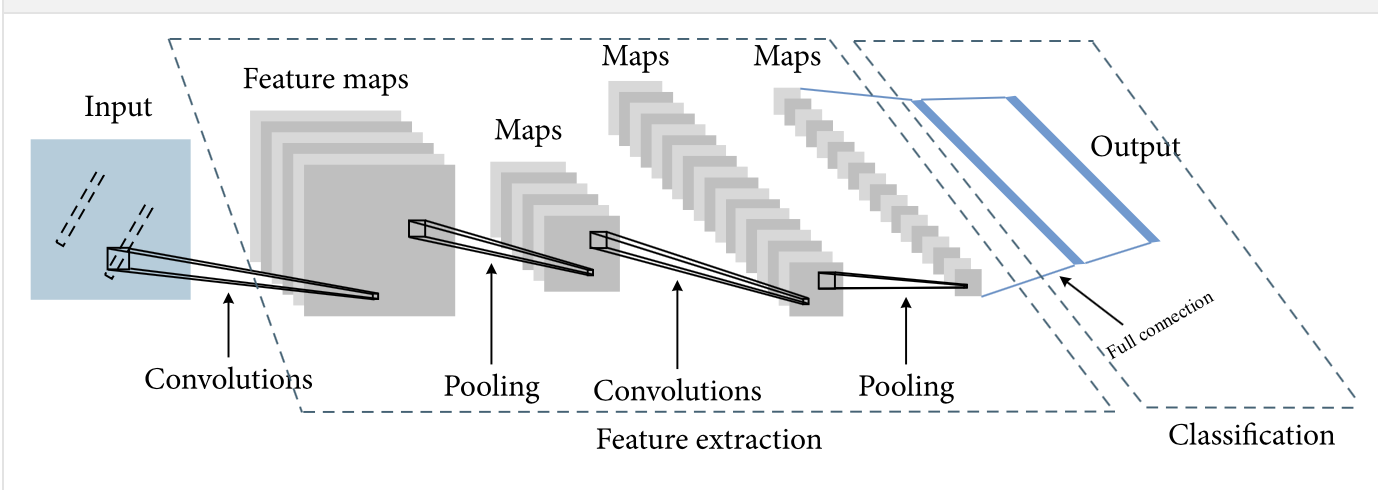
\includegraphics[scale=.7]{res/image2.png}}
	\caption{Архітектура нейронної сгорткової нейронної мережі, яка використовувалась для аналізу данних з Літ [\ref{lit:report2}] CNN на Рис \ref{fig1}}
	\label{fig2}
\end{figure}
\begin{figure}[!h]
	\centerline{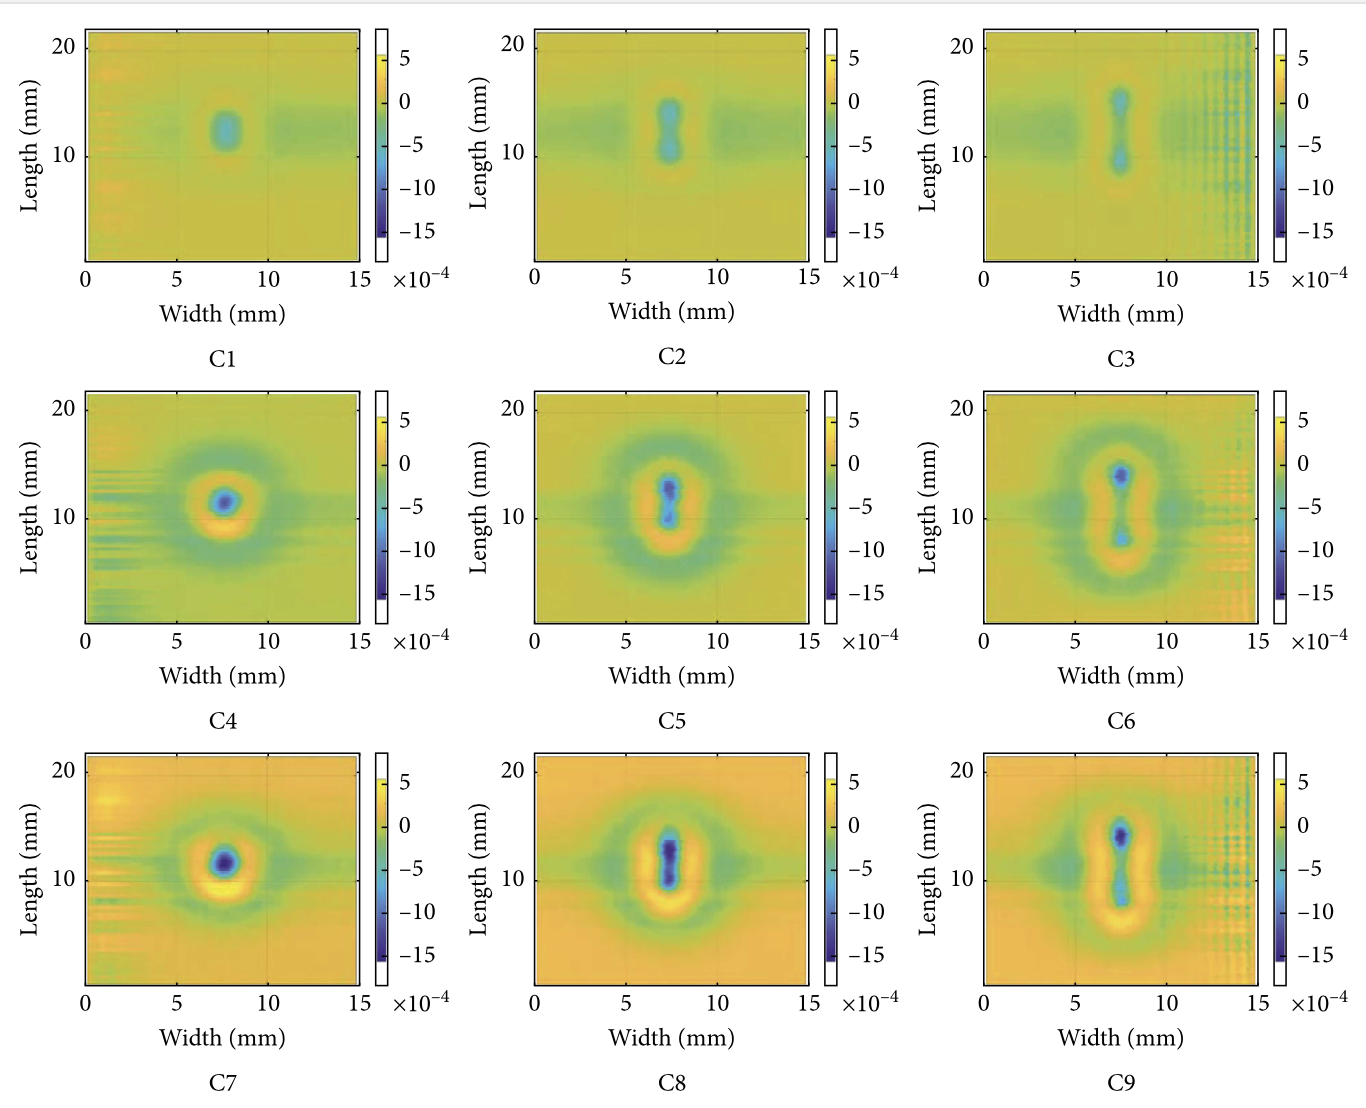
\includegraphics[scale=.7]{res/image3.png}}
	\caption{Дані вихрострумового контролю конвертовані в ргб зоображення с де частина червоного = 0, варіються лише внесок зеленого і синього}
	\label{fig3}
\end{figure}
\begin{figure}[!h]
	\centerline{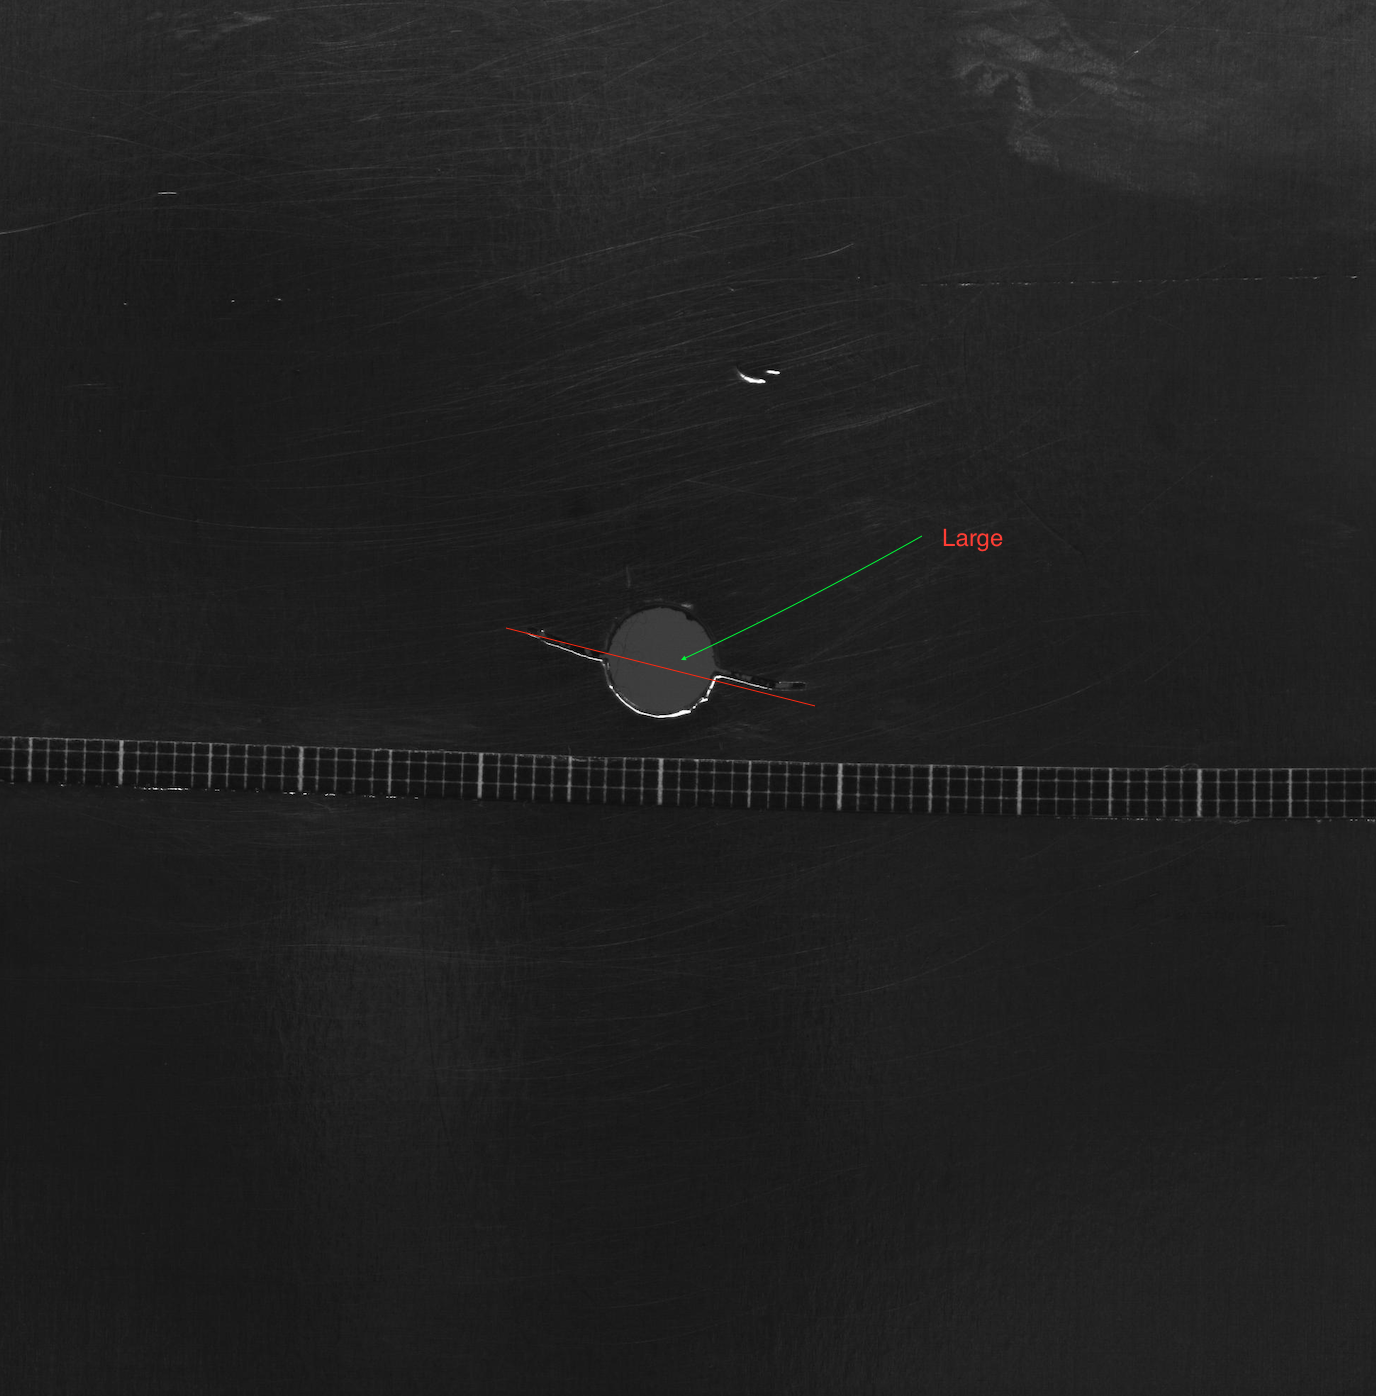
\includegraphics[scale=.7]{res/image5.png}}
	\caption{Приклад зоображення на якому навчалась мережа}
	\label{fig5}
\end{figure}

\newpage
%\section{Згорткові нейронні мережі}
%\newpage
%\section{Переваги згорткових мереж}
%\newpage
%\section{Використання для аналізу данних вихрострумового контролю}
%newpage

%literature
\addcontentsline{toc}{section}{Література}
\begin{thebibliography}{}
  
\bibitem{1}\textit{Vincentius EWALD, Xavier GOBY, Hidde JANSEN, Roger M. GROVES, Rinze BENEDICTUS 
Aerospace Non-Destructive Testing Laboratory, Faculty of Aerospace Engineering, Delft University of Technology, Delft, Netherlands
Structural Integrity and Composites Group, Delft University of Technology, Faculty of Aerospace Engineering, Delft, Netherlands} Incorporating Inductive Bias into Deep Learning: A Perspective from Automated Visual Inspection in Aircraft Maintenance \label{lit:report1}

\bibitem{1}\textit{Faculty of Mechanical and Electrical Engineering, Kunming University of Science and Technology, Kunming 650500, China
Faculty of Information Engineering and Automation, Kunming University of Science and Technology, Kunming 650500, China
Yunnan Key Laboratory of Artificial Intelligence, Kunming University of Science and Technology, Kunming 650500, China} Defect Image Recognition and Classification for Eddy Current Testing of Titanium Plate Based on Convolutional Neural Network \label{lit:report2}
\end{thebibliography}
%end

\end{document}